\begin{surferPage}[Барт]{Секстика Барта}
    Эта поверхность шестого порядка (поэтому она и названа секстикой) была сконструирована Вольфом Бартом в 1996 году.
    
У секстики Барта всего $65$ сингулярностей. Это – максимально возможное количество сингулярностей на одной секстике, как было доказано Йаффе и Руберманом, мировой рекорд Барта невозможно побить!


Конструкция Барта стала большим сюрпризом, т.к. долгое время предполагали, что поверхности шестого порядка могут иметь лишь $64$ сингулярности.

Бросается в глаза подобная икосаэдру симметрия конструкции (изображение демонстрирует икосаэдр и плоскости симметрии):
  \begin{center}
      \vspace*{-0.1cm}
      \begin{tabular}{@{}c@{\ \ }c@{\,}c@{}}
        \begin{tabular}{@{}c}
          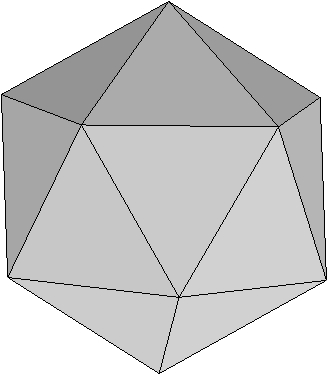
\includegraphics[width=1.4cm]{./../../common/images/icosah}
        \end{tabular}
        &
        \begin{tabular}{@{}c}
          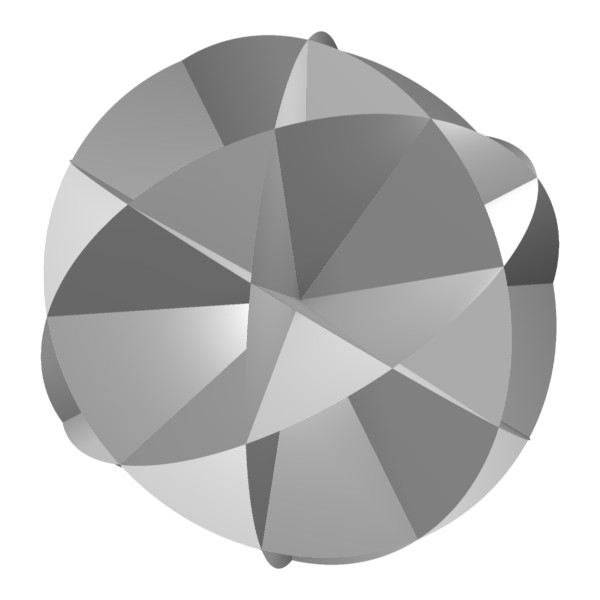
\includegraphics[width=1.4cm]{./../../common/images/barth_sextic_planes}
        \end{tabular}
        &
        \begin{tabular}{c@{}}
          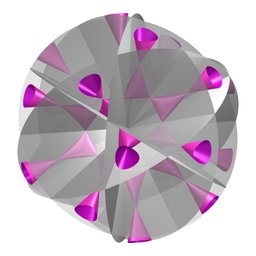
\includegraphics[width=1.4cm]{./../../common/images/barth_sextic_and_planes}
        \end{tabular}
      \end{tabular}
    \end{center}
    \vspace*{-0.1cm}

	Секстика Барта соответствует уравнению:
    $P_6 - \alpha K^2=0,$ , при этом $P_6$
    определяет плоскости симметрии, $K=x^2+y^2+z^2-1$ - сферу, а
    $\alpha=\frac{1}{4}(2+\sqrt{5})$.
\end{surferPage}
